\documentclass[tikz,border=3.14mm]{standalone}
\usepackage{pgfplots}
\usetikzlibrary{backgrounds,matrix,fit,calc}
\pgfplotsset{compat=1.16}
\definecolor{metropolisorange}{RGB}{235,129,27}

\pgfplotsset{
colormap={whitered}{color(0cm)=(white); rgb255(1cm)=(235,129,27)}
}

\begin{document}
	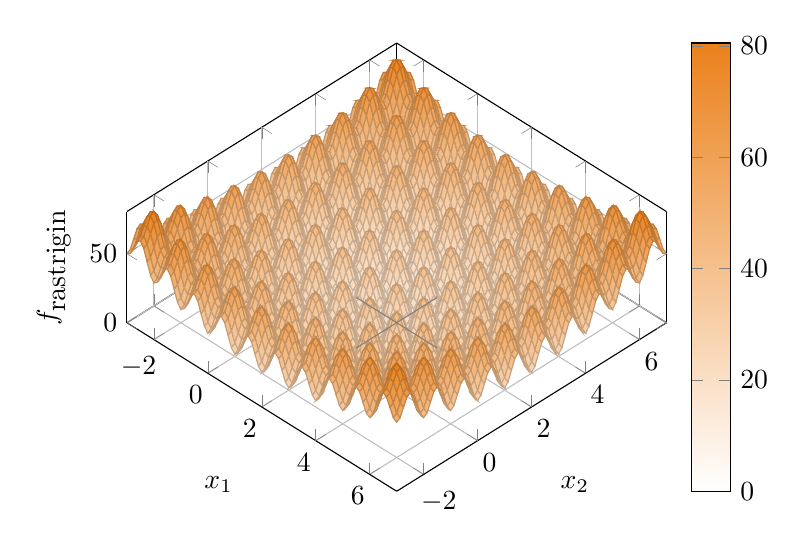
\begin{tikzpicture}[
	  declare function={rastrigin=20 + ((x-2)^2 - 10*cos(deg(2.0*pi*(x-2)))) + ((y-2)^2 - 10*cos(deg(2.0*pi*(y-2))));}, scale=1.0]
	  \begin{axis}[
		colormap name=whitered,
		view={45}{65},
		enlargelimits=false,
		grid=major,
		domain=-3:7,
		y domain=-3:7,
		samples=81,
		xlabel=$x_1$,
		ylabel=$x_2$,
		zlabel={$f_{\textrm{rastrigin}}$},
		colorbar,
		]
		\addplot3 [surf] {rastrigin};
		\draw [black!50] (axis cs:0.5,2,0) -- (axis cs:3.5,2,0);
		\draw [black!50] (axis cs:2,0.5,0) -- (axis cs:2,3.5,0);
	  \end{axis}
	\end{tikzpicture}
\end{document}
